\documentclass[numerate]{cheatsheet}
\usepackage{bm}
\usepackage{textcomp, mathcomp}
\usepackage{empheq}
\usepackage{pbox}
\usepackage{booktabs}

\doctitle{Thermodynamics III Cheatsheet}
\author{Christian Leser (cleser@ethz.ch) \\ \vspace*{-0.2em}}

\begin{document}
\section{Conduction}
	\subsection{Definition}
    Heat transfer in a body due to temperature difference
	\subsection{Fouriers Law}
    \begin{minipage}{0.49\linewidth}
        \begin{empheq}[box = \fbox]{align*}
            &\vec{\dot{q}}'' = -\lambda \nabla T\\
            \text{1D:} \quad & \dot{q_x}'' = \frac{\dot{Q}}{A}= -\lambda \frac{dT}{dx}
        \end{empheq}
    \end{minipage}
    \begin{minipage}{0.49\linewidth}
        \begin{scriptsize}
            \begin{empheq}{align*}
                \vec{\dot{q}}'' = \text{Heat flux}, \left[\frac{W}{m^2}\right]\\
                \lambda = \text{thermal conductivity}, \left[\frac{W}{m K}\right]\\
            \end{empheq}
        \end{scriptsize}
    \end{minipage}

    3-Dimensional equations follow the fouriers and fick's law:
    \begin{empheq}[box = \fbox]{align*}
        \vec{\dot{q}}'' &= \underbrace{-\lambda \frac{\partial T}{\partial x} \hat{x}}_{\dot{q}_x''} \underbrace{-\lambda \frac{\partial T}{\partial y} \hat{y}}_{\dot{q}_y''} \underbrace{-\lambda \frac{\partial T}{\partial z} \hat{z}}_{\dot{q}_z''}\\
        \vec{\dot{q}}'' &= \underbrace{-\lambda \frac{\partial T}{\partial r} \hat{r}}_{\dot{q}_r''} \underbrace{-\lambda \frac{\partial T}{r \partial \phi} \hat{\phi}}_{\dot{q}_\phi''} \underbrace{-\lambda \frac{\partial T}{\partial z} \hat{z}}_{\dot{q}_z''}\\
        \vec{\dot{q}}'' &= \underbrace{-\lambda \frac{\partial T}{\partial r} \hat{r}}_{\dot{q}_r''} \underbrace{-\lambda \frac{\partial T}{r \partial \theta} \hat{\theta}}_{\dot{q}_\theta''} \underbrace{-\lambda \frac{\partial T}{r \sin(\theta) \partial \phi} \hat{\phi}}_{\dot{q}_\phi''}
    \end{empheq}
    \textbf{Koordinatensysteme Zylindrisch und Sphärisch}

    \titel{Some common thermal conductivities}
    \begin{tabular}{c c}
        \textbf{Material} & \textbf{thermal conductivity $ \lambda \left[\frac{W}{mK}\right]$}\\
        Aluminium: & 240\\
        Copper: & 400\\
        Carbon steels: & 40-60\\
        Stainless steels: & 15\\
        Helium: & 0.152\\
        Air or $N_2$: & 0.026\\
        Steam (100°C): & 0.025\\
        Plastic: & 0.2\\
        Rubber: & 0.16\\
    \end{tabular}
	\subsection{Heat Conduction Equation}
    \begin{empheq}{align*}
        \text{Remember:} \quad
        \nabla = 
        \begin{bmatrix}
            \frac{\partial}{\partial x}\\
            \frac{\partial}{\partial y}\\
            \frac{\partial}{\partial z}
        \end{bmatrix}
    \end{empheq}

    \begin{empheq}[box = \fbox]{align*}
        &\underbrace{\rho c \frac{\partial T}{\partial t}}_{\substack{\text{th. energy flow}\\ \text{into control volume}}} = \underbrace{\vec{\nabla} \left(\lambda \vec{\nabla} T\right)}_{\substack{\text{Change in thermal} \\ \text{energy storage}}} + \underbrace{\dot{Q}_{\text{source}}'''}_{\substack{\text{Thermal energy} \\ \text{generation}}}\\
        &= \frac{\partial}{\partial x} \left(\lambda \frac{\partial T}{\partial x}\right) + \frac{\partial}{\partial y} \left(\lambda \frac{\partial T}{\partial y}\right) + \frac{\partial}{\partial z} \left(\lambda \frac{\partial T}{\partial z}\right) + \dot{Q}_{\text{source}}'''\\
        &= \frac{1}{r} \frac{\partial}{\partial r} \left(\lambda r \frac{\partial T}{\partial r}\right) + \frac{1}{r^2} \frac{\partial}{\partial \varphi} \left(\lambda \frac{\partial T}{\partial \varphi}\right) + \frac{\partial}{\partial z} \left(\lambda \frac{\partial T}{\partial z}\right) + \dot{Q}_{\text{source}}'''\\
        &= \frac{1}{r^2} \frac{\partial}{\partial r} \left(\lambda r^2 \frac{\partial T}{\partial r}\right) + \frac{1}{r^2 \sin^{\theta}} \frac{\partial}{\partial \varphi} \left(\lambda \frac{\partial T}{\partial \varphi}\right) + \frac{1}{r^2 \sin(\theta)} \frac{\partial}{\partial \theta} \left(\lambda \sin(\theta) \frac{\partial T}{\partial \theta}\right) + \dot{Q}_{\text{source}}'''
    \end{empheq}
    
    \subsubsection{Solving the Heat Conduction Equation: Boundary conditions \textbf{(Noch machen, Lecture 2 oder 3)}}
        \begin{itemize}
            \item Surface Temperature known
            \item Heat Flux known
            \item Convection known
        \end{itemize}

\section{Convection}
	\subsection{Heat transfer by convection}
\begin{minipage}{0.49\linewidth}
    \begin{empheq}[box = \fbox]{align*}
        \dot{q}'' = \frac{\dot{Q}}{A} = \alpha (T_{\infty} - T_W)
    \end{empheq}
\end{minipage}
\begin{minipage}{0.49\linewidth}
    \begin{scriptsize}
        \begin{empheq}{align*}
            \vec{\dot{q}}'' = \text{Heat flux}, \left[\frac{W}{m^2}\right]\\
            \alpha = \text{heat transfer coefficient}, \left[\frac{W}{m K}\right]\\
        \end{empheq}
    \end{scriptsize}
\end{minipage}

\section{Thermal Resistances}
	\subsection{Thermal resistance model}
    assumption: $\lambda = const$
    \begin{empheq}{align*}
        \dot{Q_x} = \dot{Q_x}'' A = \frac{1}{R_{th}} \Delta T\\
    \end{empheq}

    \begin{tabular}{c c c}
        \textbf{Geometry} & \textbf{Conduction $R_{th}$} & \textbf{Convection $R_{th}$}\\
        Planar & $\frac{L}{\lambda A}$ & $\frac{1}{\alpha A}$ \\
        Cylinder & $\frac{\ln\left(\frac{r_2}{r_1}\right)}{2 \pi \lambda L}$ & $\frac{1}{2 \pi r_1 L \alpha}$ \\
        Sphere & $\frac{\frac{1}{R_1} - \frac{1}{R_2}}{4 \pi \lambda}$ & $\frac{1}{4 \pi r^2 \alpha}$ \\
    \end{tabular}

    Note that for some pipes, there exists a critical thickness of the pipe insulation, for which the thermal insulation of a thin insulation layer is lower than without insulation layer.\\
    $R_{crit}: \frac{d}{dr_2} (R_{tot}) = 0, R_{tot} = R_{th, ins} + R_{th, conv}$\\
    $\Rightarrow r_{2, crit} = \frac{\lambda}{\alpha}$

\section{Lumped capacitance method}
	\subsection{Lumped capacitance}
    \begin{minipage}{0.39 \linewidth}
        Idea: The temperature in a body is almost uniform, so we can assume it to be uniform.
        Temperature within body will now be $T(t)$ instead of $T(t, x, y, z)$.
        That means, the temperature difference inside the body $\Delta T_i = T_{s, 1} - T_{s, 2}$ must be much smaller than the temperature difference outside the body $\Delta T_o = T_{s, 2} - T_{\infty}$.
    \end{minipage}
    \begin{minipage}{0.59 \linewidth}
        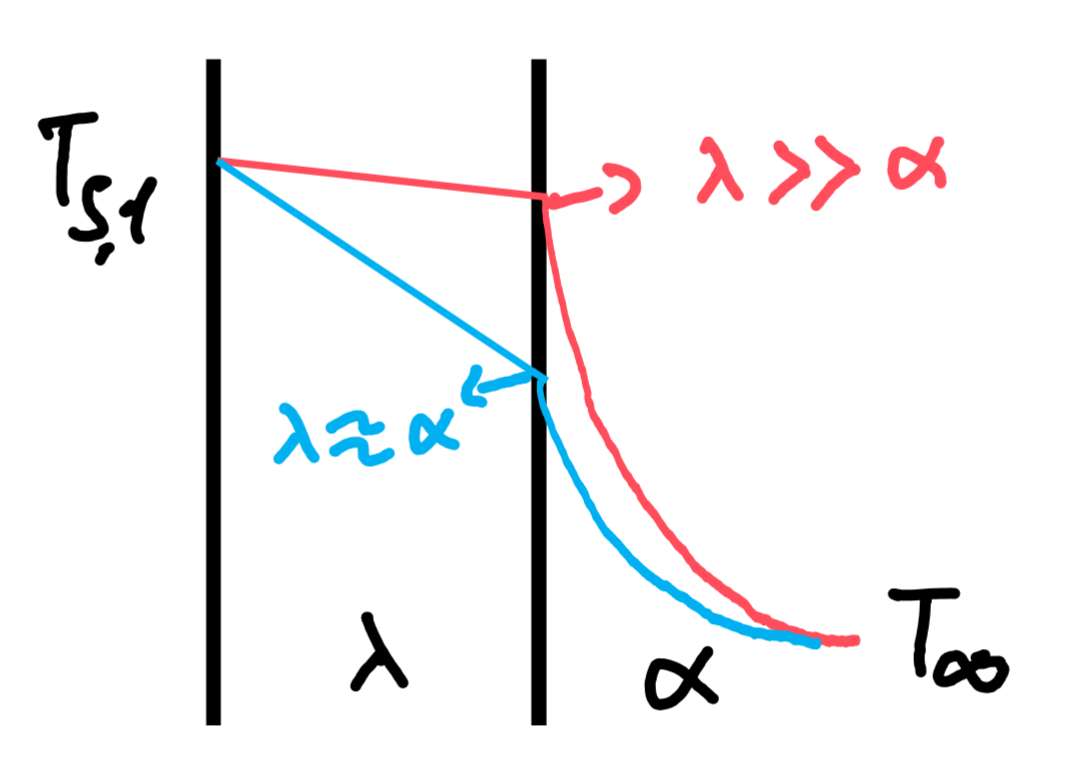
\includegraphics[width = \linewidth]{src/images/lumped_cap.png}
    \end{minipage}

    \begin{empheq}{align*}
        \dot{q} = \frac{\lambda A}{L} (T_{s, 1} - T_{s, 2}) = \alpha A (T_{s, 2} - T_{\infty})\\
        \Rightarrow \frac{(T_{s, 1} - T_{s, 2})}{(T_{s, 2} - T_{\infty})} = \frac{\alpha L}{\lambda} = Bi\\
        L_{\text{cylinder}} = \frac{r}{2} \quad \quad L_{\text{sphere}} = \frac{r}{3}
    \end{empheq}

% Continue with lecture 5
\end{document}